\documentclass[class=book, crop=false, oneside, 12pt]{standalone}
\usepackage{standalone}
\usepackage{amsmath}
\usepackage{../../style}
\graphicspath{{./assets/images/}}

% arara: pdflatex: { synctex: yes, shell: yes }
% arara: latexmk: { clean: partial }
\begin{document}

\chapter{Secondo principio della Termodinamica}

\section{Enunciati del secondo principio della termodinamica}

Il primo principio della termodinamica non pone limiti alle trasformazioni di energia da una forma all'altra, però la situazione sperimentale non appare simmetrica: mentre è sempre possibile trasformare integralmente lavoro in calore, per esempio sfruttando l'attrito, la trasformazione contraria di calore in lavoro sembra essere limitata, indipendentemente dal primo principio.

\subsection{Esempio: macchina termica}

Prendiamo in esame il caso di una macchina che compie un ciclo termico scambiando calore con due sorgenti. 
Si verifica che il calore scambiato complessivamente dal sistema, che viene utilizzato per far funzionare la macchina \(M\), con le due sorgenti di calore alle temperature \(T_1\) e \(T_2\) (\(T_2 > T_1\) ) è dato dalla somma di una quantità \(Q_A\), assorbita dalla sorgente a temperatura maggiore, e di una quantità \(Q_C\), ceduta alla sorgente a temperatura minore. 
Si osserva che è sempre \(Q_C<0\), cioè non succede mai \(Q_C \geq 0\). 
Questo risultato comporta che \(Q_A\) non viene trasformato integralmente in lavoro, ma una parte \(Q_C\) viene sempre ceduta alla sorgente a temperatura inferiore. 
Il lavoro è \(W = Q_A + Q_C\) e in accordo con il primo principio (\(\Delta U = 0\) in un processo ciclico), però non si ha mai \(W = Q_A\), bensì \(W < Q_A\). 

Nel caso ci siano più sorgenti con cui la macchina \(M\) scambia calore la situazione è analoga: la somma dei calori assorbiti non si trasforma mai totalmente in lavoro, una parte viene sempre ceduta restando cioè sotto forma di calore scambiato. 
Non esistono esempi contrari: in un processo ciclico vi è una impossibilità di trasformazione integrale di calore in lavoro ovvero la trasformazione di calore in lavoro è sempre accompagnata da cessione di calore. 

Accanto all'impossibilità finora discussa esiste un'altra impossibilità sperimentale. 
Se consideriamo due corpi a temperatura diversa e li mettiamo a contatto termico, c'è sempre una cessione di calore dal corpo caldo al corpo freddo fino a che si raggiunge l'equilibrio termico. 

\emph{Il calore non passa mai spontaneamente dal corpo freddo al corpo caldo}. 
È possibile fare avvenire questo passaggio, come si realizza in una macchina frigorifera, ma deve essere eseguito un lavoro sulla sostanza che compie il ciclo.

\subsection{Enunciati}

Il secondo principio della termodinamica consiste nel prendere atto di queste impossibilità sperimentali, che non presentano eccezioni conosciute, e  nel trasformarle in postulati, secondo i seguenti enunciati. 

Enunciato di \emph{Kelvin-Planck}\newline
\emph{È impossibile realizzare un processo che abbia come unico risultato la trasformazione in lavoro del calore fornito da una sorgente a temperatura uniforme.}

Enunciato di \emph{Clausius}\newline
\emph{È impossibile realizzare un processo che abbia come unico risultato il trasferimento di una quantità di calore da un corpo ad un altro a temperatura maggiore. }

L'aggettivo unico utilizzato nei due enunciati è essenziale: abbiamo infatti già visto negli esempi dell'espansione isoterma di un gas ideale e del ciclo frigorifero che i processi proibiti dal secondo principio sono possibili, se non costituiscono l'unico risultato. 
Conseguenza immediata del secondo principio, nell'enunciato di Kelvin-Planck, sono i fatti già evidenziati: in un processo ciclico per produrre effettivamente lavoro sono necessarie sempre almeno due sorgenti, cioè non può sussistere il risultato \(Q_C = 0\), ma deve essere \(Q_A > |Q_C|\) e quindi, \(\eta < 1\).

\subsection{Equivalenza degli enunciati}

Gli enunciati di Kelvin-Planck e di Clausius, pur se riferiti a fatti sperimentali che appaiono molto diversi, sono strettamente connessi in quanto se fosse possibile realizzare uno dei processi proibiti sarebbe possibile realizzare anche l'altro.

\subsubsection*{Kelvin-Planck \(\implies\) Clausius}

\begin{figure}[h] 
    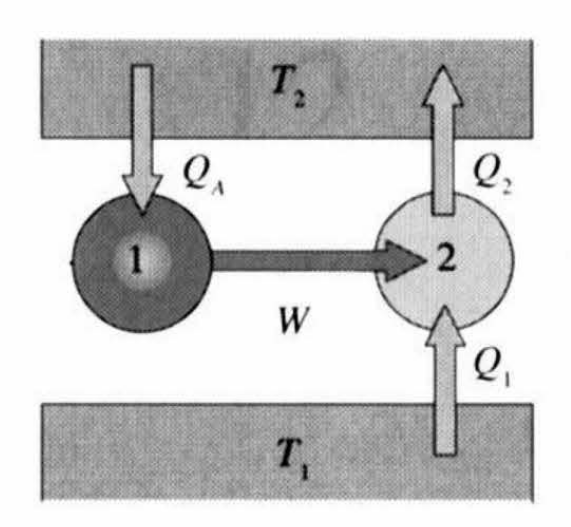
\includegraphics[scale=0.4]{not_kelvin.png}
    \centering
    \caption{}
    \label{not_kelvin}
\end{figure}
Supponiamo infatti che sia possibile realizzare un processo ciclico che trasformi integralmente calore in lavoro, in contrasto con l'enunciato di Kelvin-Planck. 
Questo fatto è rappresentato nella figura (\ref{not_kelvin}), dove la macchina termica \(1\) produce il lavoro \(W\) trasformando il calore \(Q_A\) assorbito dalla sorgente a temperatura \(T_2 : W = Q_A\) ed è nulla la cessione di calore alla sorgente fredda. 
Utilizziamo il lavoro \(W\) per far funzionare una macchina frigorifera, che preleva il calore \(Q_1\) dalla sorgente a temperatura \(T_1\) e cede il calore \(Q_2\) alla sorgente a temperatura \(T_2>T_1\). 
Questa seconda macchina non contraddice l'enunciato di Clausius dato che nel processo interviene il lavoro \(W^{\prime} = -W\) fatto sul sistema (il lavoro \(W\) è fatto dalla macchina \(1\) ed è positivo, mentre \(W^{\prime}\) è subito dalla macchina \(2\) ed è negativo: 
le due quantità sono eguali in modulo, ma opposte in segno). 
Il bilancio della macchina \(2\), sulla base del primo principio, è 
\begin{equation*}
    Q_1 + Q_2 = W^{\prime} = - W.
\end{equation*}
La macchina complessiva, costituita dall'insieme delle due macchine, assorbe \(Q_1\) a temperatura \(T_1\) e scambia a temperatura \(T_2\). 
Se \(Q_1\) è assorbito, \(-Q_1\) è ceduto. 
Il lavoro complessivo della macchina è nullo in quanto non c'è scambio di lavoro con l'ambiente esterno e l'unico risultato pertanto è il passaggio spontaneo di calore dalla sorgente a temperatura inferiore a quella a temperatura superiore, violando l'enunciato di Clausius.

\subsubsection*{Clausius \(\implies\) Kelvin-Planck}

\begin{figure}[h]
    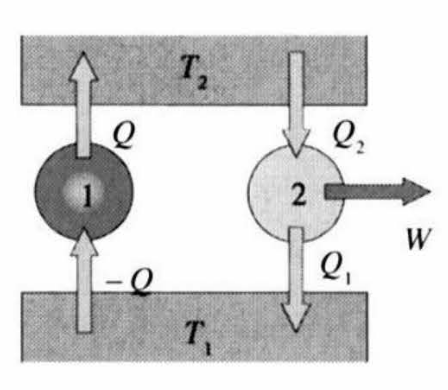
\includegraphics[scale=0.4]{not_clausius.png}
    \centering
    \caption{}
    \label{not_clausius}
\end{figure}

Supponiamo ora di poter realizzare una macchina che come unico risultato faccia passare il calore \(Q\) da una sorgente a temperatura \(T_1\) ad un'altra a temperatura \(T_2 > T_1\) e consideriamo una seconda macchina che lavori normalmente tra le due sorgenti, in accordo col secondo principio (figura \ref{not_clausius}). 
Dimensioniamo questa seconda macchina in modo che \( Q_1 = Q\), cioè in modo da cedere alla sorgente a \(T_1\) lo stesso calore che viene assorbito dalla prima macchina.
Pertanto alla fine di un ciclo della macchina complessiva la sorgente a \(T_1\) non scambia calore e il lavoro prodotto è dato da 
\begin{equation*}
    W = Q_2 + Q_1 = Q_2 + Q
\end{equation*}
ed è positivo, perché \(Q_2 > |Q_1| = |Q| \); tale lavoro è eguale al calore complessivamente scambiato con la sorgente a \(T_2\) e in conclusione l'unico risultato è la trasformazione integrale in lavoro del calore assorbito da una sola sorgente (a temperatura \(T_2\) ), violando l'enunciato di Kelvin-Planck.

L'unione dei risultati ottenuti costituisce la cosiddetta equivalenza tra i due enunciati del secondo principio della termodinamica nel senso che abbiamo visto: la negazione di uno ha come conseguenza la negazione dell'altro.

\section{Reversibilità e irreversibilità}

Quando viene compiuta una trasformazione reversibile da uno stato \(A\) ad uno stato \(B\), con scambio della quantità \(Q_{AB}\) e \(W_{AB}\) tra il sistema e l'ambiente, è sempre possibile ripercorrerla in senso inverso, scambiando le quantità \(-Q_{AB}\) e \(-W_{AB}\): alla fine sistema e ambiente sono ritornati ai rispettivi stati iniziali, dato che lo scambio totale di calore e lavoro è nullo per entrambi. 
L'argomento si estende ai cicli reversibili: alla fine di un ciclo il sistema torna sempre nello stato iniziale, ma l'ambiente ha subito una modifica perché ha, per esempio, ceduto calore e assorbito lavoro. 
Percorrendo il ciclo in senso inverso gli scambi energetici dell'ambiente sono eguali ed opposti ed esso ritorna nello stato iniziale.

In generale: \emph{una trasformazione reversibile non comporta alterazioni permanenti, nel senso che è sempre possibile riportare nei rispettivi stati iniziali il sistema e l'ambiente che con esso interagisce}

La situazione è completamente diversa per le trasformazioni irreversibili:
\begin{enumerate}
    \item Presenza durante il processo di effetti dissipativi dovuti alle forze di attrito, come avviene nello spostamento del pistone di un cilindro contenente un gas: contro le forze di attrito viene speso un certo lavoro \(W\) che alla fine ritroviamo trasformato integralmente in calore \(Q\) ceduto all'ambiente. 
    Questo calore \(Q\) non può essere ritrasformato integralmente in lavoro: si è verificata una modifica permanente. 
    \item Espansione libera di un gas: in essa \(Q = W = 0\). 
    Alla fine della trasformazione, se vogliamo riportare il gas nello stato iniziale possiamo utilizzare una compressione isoterma reversibile, che richiede un lavoro esterno. 
    Il gas viene riportato nello stato iniziale, ma l'ambiente ha subito una modifica che non si può più recuperare. 
    \item Passaggio di calore tra due corpi a contatto termico e che presentano una differenza finita di temperatura: alla fine si raggiunge l'equilibrio termico, senza produzione di lavoro, ma per ripristinare la situazione iniziale si dovrebbe fornire lavoro dall'esterno, per esempio utilizzando una macchina frigorifera reversibile.
\end{enumerate}
Da questi, e da qualsiasi altro esempio, si \emph{conclude che quando avviene una trasformazione irreversibile non è più possibile ritornare allo stato di partenza senza modificare il resto dell'universo}. 
Il sistema può essere riportato allo stato iniziale attraverso altre trasformazioni, ma l'ambiente subisce una modifica irreversibile.

Le considerazioni esposte sono importanti perché nella pratica tutte le trasformazioni che avvengono in natura contengono fattori di irreversibilità.  
La rappresentazione di un fenomeno reale con una trasformazione reversibile costituisce quindi una idealizzazione del processo che permette di eseguire calcoli altrimenti impossibili e avere stime sulle grandezze in gioco, spesso sotto forma di limiti superiori.

\section{Teorema di Carnot}

Il teorema di Carnot rappresenta una prima precisazione quantitativa dell'enunciato di Kelvin-Planck in quanto fissa la massima percentuale di calore assorbito da una macchina termica che può essere trasformata in lavoro.

Consideriamo due macchine che lavorano utilizzando le stesse sorgenti di calore alle temperature \(T_1\) e \(T_2>T_1\), dimensionate in modo tale da produrre lo stesso lavoro. 
Indichiamo le due macchine con i simboli \(X\) e \(R\): per la prima macchina non facciamo per ora alcuna ipotesi di reversibilità o irreversibilità, mentre assumiamo che la seconda sia reversibile. 
I rendimenti delle due macchine sono, data l'ipotesi sul lavoro,
\begin{equation*}
    \eta_X = \frac{W}{Q_2} \ , \ \eta_R = \frac{W}{Q^{\prime}_2}
\end{equation*}
Dal primo principio abbiamo inoltre:
\begin{equation}
    Q_2 + Q_1 = W = Q_1^{\prime} + Q_2^{\prime}
\end{equation}

Supponiamo che sia \(\eta_X > \eta_R\) e costruiamo una macchina composta da \(X\) e \(R\), in cui quest'ultima viene fatta funzionare come macchina frigorifera, assorbendo il lavoro \(-W\) e il calore \(-Q^{\prime}_1\) e cedendo il calore \(-Q_2^{\prime}\):
sfruttiamo così una proprietà caratteristica di un processo reversibile come è stato ipotizzato.

Dall'ipotesi segue:
\begin{equation*}
    \frac{W}{Q_2} > \frac{W}{Q_2^{\prime}} \Leftrightarrow Q_2 < Q_2^{\prime} \Leftrightarrow Q_2 - Q_2^{\prime} < 0
\end{equation*}
e quindi da (8.1)
\begin{equation*}
    Q_1 - Q_1^{\prime} = Q_2^{\prime} - Q_2 > 0 
\end{equation*}

Abbiamo complessivamente i seguenti risultati:
\begin{enumerate}
    \item la macchina assorbe il calore \(Q = Q_1 -Q_1^{\prime}> 0\) dalla sorgente a temperatura \(T_1\);
    \item non viene scambiato calore con l'esterno
    \item la macchina cede il calore \(-Q = Q_2 - Q_2^{\prime} < 0 \) alla sorgente a temperatura \(T_2\).
\end{enumerate} 
L'unico risultato alla fine di un ciclo è il passaggio di calore dalla sorgente fredda alla sorgente calda, in contrasto con l'enunciato di Clausius. 
Allora è sbagliata l'ipotesi di partenza e deve essere
\begin{equation}
    \eta_X \leq \eta_R
\end{equation}

Se anche la macchina \(X\) fosse reversibile, potremmo supporre \(\eta_R > \eta_X\), far funzionare la macchina \(X\) come macchina frigorifera (calore e lavoro cambierebbero solo di segno dato \(X\) reversibile)
e troveremmo \(\eta_X \geq \eta_R\).
Le disuguaglianze sono compatibili solo se
\begin{equation} \label{teorema_carnot}
    \eta_X = \eta_R
\end{equation}

In conclusione il \emph{Teorema di Carnot} afferma che tutte le macchine reversibili che lavorano tra le stesse sorgenti alle temperature \(T_1\) e \(T_2\) hanno rendimento eguale; qualsiasi altra macchina che lavori tra le stesse sorgenti non può avere rendimento maggiore. 
Il risultato è indipendente dal particolare sistema che compie il ciclo, come si deduce dal fatto che le proprietà del sistema non compaiono nella dimostrazione.

Da (\ref{teorema_carnot}) deduciamo allora che il rendimento del \emph{ciclo di Carnot a gas ideale} rappresenta il rendimento di tutte le macchine reversibili che lavorano con due sole sorgenti alle temperature \(T_1\) e \(T_2\).
Il teorema di Carnot risulta valido anche per macchine che lavorano con più sorgenti, non esiste però una formula generale come quella vista prima.

Ritornando al caso di due sorgenti si ha che, per qualsiasi macchina reversibile, la relazione tra calori scambiati e temperature a cui avviene lo scambio è
\begin{equation} \label{rel_q_temp}
    \frac{Q_1}{T_1} + \frac{Q_2}{T_2} = 0
\end{equation}
Ricordiamo che \(T\) è la temperatura misurata col termometro a gas ideale. 
Fissate dunque le temperature delle sorgenti, \(T_1\) e \(T_2\), con \(T_2 > T_1\), per il teorema di Carnot
\begin{equation}
    \eta_R = \eta_{max} = 1- \frac{T_1}{T_2}
\end{equation}
la macchina reversibile è quella che sfrutta meglio l'energia fornitale sotto forma di calore.
Infatti a parità di calore assorbito \(Q_A\), la macchina reversibile è quella che fornisce il lavoro massimo, 
\begin{equation}
    W_{max} = Q_A \eta_R = Q_A \left(1 - \frac{T_1}{T_2}\right) = T_1 \left(\frac{Q_A}{T_1} - \frac{Q_A}{T_2}\right)
\end{equation}
ovvero, \emph{a parità di lavoro fornito, la macchina reversibile è quella che assorbe meno calore}.
\begin{equation}
    Q_{min} = \frac{W}{\eta_R} = \frac{W}{1- \frac{T_1}{T_2}}
\end{equation}

\section{Teorema di Clausius}

La relazione (\ref{rel_q_temp}), conseguenza del teorema di Carnot per le macchine reversibili che lavorano tra due sorgenti, può essere estesa e generalizzata a macchine termiche operanti con più sorgenti di calore. 

\subsection{Enunciato}

Data una macchina \(M\) qualsiasi la quale scambia calore con \(n\) sorgenti, sussiste la relazione 
\begin{equation} \label{enunciato_teorema_clausius}
    \sum_{i = 1}^{n} \frac{Q_i}{T_i} \leq 0
\end{equation}
dove \(Q_1, Q_2, ... , Q_n\) sono i calori scambiati con le sorgenti a temperatura \(T_1, T_2, ... , T_n.\)
\begin{figure}[h]
    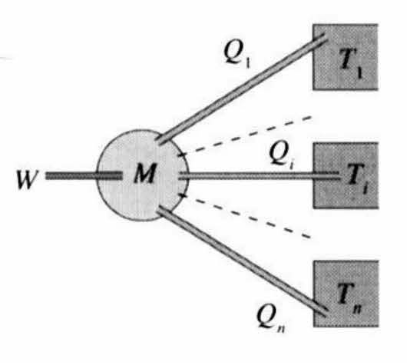
\includegraphics[scale=0.4]{clausius_enunciato.png}
    \centering
    \caption{}
\end{figure}

\subsection{Dimostrazione}

Per dimostrare il teorema di Clausius, immaginiamo di aggiungere \(n\) macchine reversibili funzionanti tra le sorgenti già considerate alle temperature \(T_1 , T_2 , ... , T_n\) e una sorgente a temperatura \(T_0\): ciascuna di queste macchine \(R_i\); scambia con la sorgente a \(T_i\); il calore \(-Q_i\), opposto a quello scambiato con la stessa sorgente dalla macchina \(M\), e con la sorgente a \(T_0\) il calore \(Q_0\).
\begin{figure}[h]
    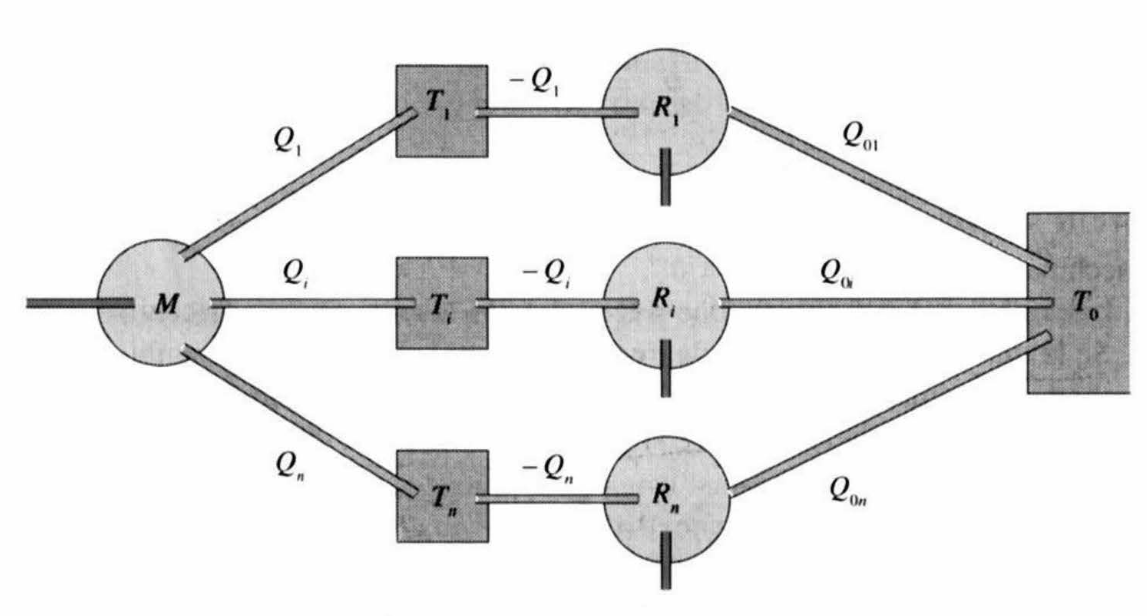
\includegraphics[scale=0.4]{clausius_dim.png}
    \centering
    \caption{}
\end{figure}
Applichiamo (\ref{rel_q_temp}) a ciacuna macchina reversibile:\\
\begin{align*}
    \text{per } &R_1 & -\frac{Q_1}{T_1} + \frac{Q_{01}}{T_0} &= 0 \implies \frac{Q_{01}}{T_0} = \frac{Q_1}{T_1} \\
    \text{per } &R_i & -\frac{Q_i}{T_i} + \frac{Q_{0i}}{T_0} &= 0 \implies \frac{Q_{0i}}{T_0} = \frac{Q_i}{T_i} \\
    \text{per } &R_n & -\frac{Q_i}{T_i} + \frac{Q_{0n}}{T_0} &= 0 \implies \frac{Q_{0n}}{T_0} = \frac{Q_n}{T_n} \\
\end{align*}

e sommando a tutte le macchine 
\begin{equation*}
    \frac{1}{T_0} \sum_i Q_{0i} = \sum_{i} \frac{Q_i}{T_i}
\end{equation*}

Alla fine di un ciclo della macchina \(M\) e delle macchine reversibili \(R_1, ... , R_n\) le sorgenti a \(T_0, ... , T_n\) sono rimaste invariate in quanto ciascuna ha scambiato calori eguali ed opposti con le macchine. 
Pertanto la macchina complessiva costituita da \(M\) e dalle \(n\) macchine ausiliarie compie una trasformazione ciclica monoterma perché scambia calore solo con la sorgente a temperatura \(T_0\).
Dato che il calore totale scambiato durante un ciclo monotermo non può essere positivo ottengo:
\begin{equation*}
    \sum_i Q_{0i} \leq 0 \implies \sum_i \frac{Q_i}{T_i} \leq 0
\end{equation*}
poichè \(T_0 > 0 \).

Se lo scambio di calore di \(M\) avviene con una serie infinita di sorgenti, detto \(d Q\) il calore scambiato con la sorgente a temperatura \(T\), la (\ref{enunciato_teorema_clausius}) diventa
\begin{equation} \label{conclusione_dim_teorema_clausius}
    \oint \frac{d Q}{T} \leq 0
\end{equation}
dove \(\oint\) indica che l'integrale è esteso a tutto il ciclo descritto dalla macchina \(M\).

\subsection{Teorema di Clausius per macchine reversibili}

Le equazioni (\ref{enunciato_teorema_clausius}) e (\ref{conclusione_dim_teorema_clausius}) esprimono il teorema di Clausius per una macchina generica.
Se la macchina \(M\) è reversibile invertiamo tutti i cicli: tutti gli scambi di calore cambiano di segno e deve essere \(\sum \left(-Q_{0i}\right) \leq 0\). 
Ne segue che le disugualianze del teorema vanno invertite e si ha compatibilità tra i due casi solo se 
\begin{equation} \label{comp_clausius_rev}
    \sum_{i = 1}^{n} \frac{Q_i}{T_i} = 0 \text{ oppure } \oint \frac{d Q}{T} = 0
\end{equation}

\subsection{Teorema di Clausius per macchine irreversibili}

Quando il processo ciclico è irreversibile, a rigore di logica vale il segno di minore o eguale; 
però, sulla base delle considerazioni sui processi irreversibili, possiamo assumere che in generale si verifica la diseguaglianza e si può scrivere il teorema di Clausius per le macchine irreversibili come
\begin{equation} \label{comp_clausius_irrev}
    \sum_{i = 1}^{n} \frac{Q_i}{T_i} < 0 \text{ oppure } \oint \frac{d Q}{T} < 0
\end{equation} 

Si tenga presente che la temperatura \(T\) nelle (\ref{comp_clausius_rev}) e (\ref{comp_clausius_irrev}) è quella della sorgente con cui avviene lo scambio di calore: essa coincide con la temperatura del sistema che compie il ciclo solo se il processo è reversibile. 
Inoltre i calori sono quelli visti dal sistema, positivi se il sistema li assorbe, negativi se li cede.

Osserviamo infine che mentre la somma dei calori cambiati, \(d Q\), è sempre diversa da zero per un ciclo che scambia lavoro, in accordo con il primo principio, quando il calore scambiato viene diviso per il valore della temperatura della sorgente con cui avviene lo scambio e si somma su tutto il ciclo, il risultato è nullo se il ciclo è reversibile e negativo negli altri casi. 

\section{La funzione di stato Entropia}
\begin{figure}[h]
    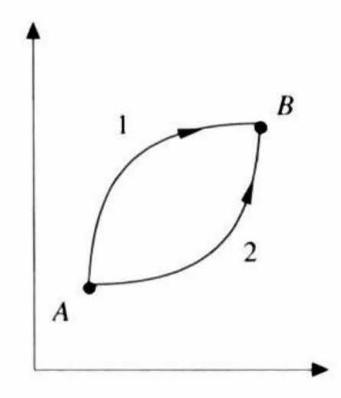
\includegraphics[scale=0.4]{trasformazioni_12.png}
    \centering
    \caption{}
    \label{trasformazione_12}
\end{figure}
Siano \(A\) e \(B\) due stati qualunque di un sistema termodinamico e passiamo da uno all'altro tramite due diverse trasformazioni reversibili.
Se percorriamo in senso inverso la trasformazione 2 (chiamandola -2), abbiamo composto un ciclo reversibile, che si svolge da A a B lungo la prima trasformazione e da B ad A lungo la seconda invertita

Dal teorema di Clausius per macchine reversibili:
\begin{equation*}
    \oint \frac{d Q}{T} = 0 = \int_A^B \left(\frac{d Q}{T}\right)_1 + \int_B^A \left(\frac{d Q}{T}\right)_{-2} = \int_A^B \left(\frac{d Q}{T}\right)_1 - \int_A^B \left(\frac{d Q}{T}\right)_{2} 
\end{equation*}
L'ultimo passaggio discende dalla proprietà delle trasformazioni reversibili secondo cui il cambio di verso nella trasformazione comporta soltanto il cambio di segno degli scambi energetici. 
Ottengo quindi
\begin{equation*}
    \int_A^B \left(\frac{d Q}{T}\right)_1 = \int_A^B \left(\frac{d Q}{T}\right)_2 = \text{ ... } = \int_A^B \left(\frac{d Q}{T}\right)_i
\end{equation*}
lungo qualsiasi trasformazione reversibile che colleghi gli stati termodinamici \(A\) e \(B\). 

Il valore dell'integrale \(\int_A^B \left(\frac{d Q}{T}\right)_{rev}\) esteso ad una qualunque trasformazione reversibile che congiunge due stati di un sistema termodinamico è sempre lo stesso, cioè non dipende dalla particolare trasformazione reversibile scelta per eseguire il calcolo. \newline
Si può quindi porre l'integrale eguale alla variazione di una funzione che dipende solo dalle coordinate termodinamiche del sistema nei due stati di equilibrio \(A\) e \(B\):
\begin{equation} \label{entropia}
    \int_A^B \left(\frac{d Q}{T}\right)_{rev(A, B)} = S_{B} - S_{A} = \Delta S_{A\rightarrow B} \udm{\frac{J}{K}}
\end{equation}
La funzione di stato così introdotta è detta \emph{entropia}.\newline
La definizione (\ref{entropia}) dà l'entropia a meno di una costante additiva arbitraria.

La definizione (\ref{entropia}) può essere scritta anche in forma infinitesima, cioè con riferimento ad una trasformazione reversibile infinitesima, che implica una variazione infinitesima delle coordinate termodinamiche:
\begin{equation} \label{entropia_infinitesima}
    d S = \left(\frac{dQ}{T}\right)
\end{equation}
\(d Q\) non è un differenziale esatto, però se tale quantità è divisa per \(T\) ed è considerata in una trasformazione reversibile, essa dà luogo al differenziale esatto \(d S\).

\emph{L'entropia è una quantità additiva}. Dati due sistemi di entropia \(S_1\) e \(S_2\), l'entropia complessiva è espressa da \(S = S_1 + S_2\).
Questa proprietà è conseguenza del fatto che l'energia interna complessiva dei due sistemi è la somma delle energie interne come pure il lavoro complessivo è la somma dei lavori, per lo meno se i sistemi sono indipendenti, pertanto anche il calore scambiato dal sistema complessivo è la somma dei calori scambiati e il risultato si estende all'entropia.
In particolare risulta che se si aumenta la massa di un sistema, l'entropia aumenta in proporzione.
L'entropia quindi ha le caratteristiche di una \emph{grandezza estensiva}.

Data una trasformazione irreversibile che collega lo stato \(A\) allo stato \(B\) di cui si vuole calcolare l'entropia, abbiamo le seguenti indicazioni:
\begin{enumerate}
    \item l'entropia dello stato iniziale e finale è certamente definibile, a partire ad esempio da un certo stato di riferimento; 
    \item conseguentemente è definibile la variazione \(S_B - S_A\) 
    \item la variazione \(S_B - S_A\) non dipende dal tipo di trasformazione che collega \(A\) e \(B\), ma solo dalle coordinate termodinamiche di \(A\) e \(B\), in quanto l'entropia è una funzione di stato. 
\end{enumerate}

Pertanto per il calcolo della variazione di entropia nella trasformazione irreversibile da \(A\) a \(B\) basta scegliere una qualsiasi trasformazione reversibile che colleghi \(A\) a \(B\) ed applicare a questa (\ref{entropia}): il risultato è valido in ogni caso.

\subsection{Diagrammi TS}

L'entropia, essendo funzione di stato, può essere scelta come variabile indipendente (coordinata termodinamica) per descrivere, insieme ad una seconda variabile indipendente opportunamente scelta (spesso \(T\)), lo stato termodinamico di un sistema.
Nel piano \(\left(T, S\right)\) una trasformazione reversibile è rappresentata da un tratto di curva continua che fornisce il grafico della funzione \(T (S)\).
Il calore scambiato dal sistema che descrive la trasformazione è, secondo (\ref{entropia_infinitesima}),
\begin{equation}
    d Q_{rev} = T ds \implies Q_{rev} = \int_A^B T d S
\end{equation}

Ne deriva che il calore scambiato nella trasformazione, assorbito se si passa da \(A\) a \(B\) (\(S_B > S_A\)), ceduto se invece si va da \(B\) ad \(A\), è dato dall'area sotto la curva \(A B\). 
Nel piano \(\left(T, S\right)\) il calore ha una semplice interpretazione grafica, come il lavoro ne piano \(\left(p, V\right)\), se le trasformazioni sono reversibili.

\subsubsection*{Trasformazioni e cicli}

Un ciclo reversibile nel piano \(\left(T, S\right)\) delimita un'area che è pari alla somma algebrica dei calori scambiati in totale del sistema, \(Q_A + Q_C\), positiva se il ciclo è percorso in senso orario negativa in caso contrario.
Tale area rappresenta anche il lavoro compiuto (primo principio).
Il rendimento di una macchina che compie un ciclo termico ha una semplice rappresentazione: esso è dato dal rapporto tra l'area racchiusa dal ciclo (\(W\)) e l'area totale sottesa dalla curva superiore \(Q_A\). 

Nel piano \(\left(T, S\right)\) una trasformazione isoterma reversibile è rappresentata da segmento orizzontale (\(T = \text{costante}\)), una trasformazione adiabatica reversibile da un segmento verticale (\(S = \text{costante}\)): infatti in tal caso \(d Q_{rev} = 0\) e, da (\ref{entropia_infinitesima}), \(d S = 0\).
Una trasformazione adiabatica reversibile è dunque isoentropica, lungo di essa l'entropia del sistema non varia.

\begin{figure}[h]
    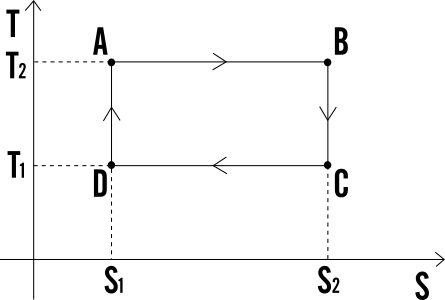
\includegraphics[scale=0.4]{ciclo-carnot-piano-t-s}
    \centering
    \caption{Ciclo di Carnot nel piano (T, S)}
\end{figure}

Un ciclo di Carnot ha la forma di un rettangolo, le formule sono:
\begin{equation*}
    Q_A = T_2 \left(S_2 - S_1\right) \ , \ Q_C = T_1 \left(S_1 - S_2\right)
\end{equation*}
\begin{equation*}
    Q = Q_A + Q_C = \left(T_2 - T_1 \right) \left(S_2 - S_1\right)
\end{equation*}
\begin{equation*}
    \eta = 1 + \frac{Q_C}{Q_A} = 1- \frac{T_1}{T_2}
\end{equation*}
Poi so che \(S_2 - S_1 = \frac{Q_A}{T_2} = \frac{-Q_C}{T_1}\):
\begin{equation*}
    W = \left(T_2 - T_1\right) \left(S_2 - S_1\right) = \left(T_2 - T_1 \right) \frac{Q_A}{T_2}
\end{equation*}

Quindi ho trovato che in una isoterma reversibile l'entropia vale
\begin{equation}
    \Delta S = \frac{Q}{T}
\end{equation}
In una adiabatica reversibile
\begin{equation}
    \Delta S = 0
\end{equation}
e che, per definizione, in una trasformazione ciclica
\begin{equation} \label{entropia_trasformazione_ciclica}
    \Delta S = 0
\end{equation}

\section{Il principio di aumento dell'entropia, Calcoli di variazione dell'entropia}

Come prima (figura \ref{trasformazione_12}) torno alle due trasformazioni 1 e 2 assumendo però che la trasformazione 1 sia irreversibile, mentre la 2 resta reversibile.

Il ciclo delle trasformazioni \(1\) e \(-2\) (\(-2\) è l'inversa della 2 come prima) rimane quindi rimane irreversibile: il teorema di Clausius ci dice:
\begin{equation*}
    \oint \frac{d Q}{T} = \int_A^B \left(\frac{d Q}{T}\right)_1 + \int_B^A \left(\frac{d Q}{T}\right)_{-2} = \int_A^B \left(\frac{d Q}{T}\right)_{irr} - \int_A^B \left(\frac{d Q}{T}\right)_{rev} < 0
\end{equation*}
L'utimo integrale rappresenta la differenza di entropia quindi:
\begin{equation}
    S_B - S_A = \int_A^B \left(\frac{d Q}{T}\right)_{rev} > \int_A^B \left(\frac{d Q}{T}\right)_{irr}
\end{equation}
Se per una generica trasformazione \(A B\) effettivamente eseguita da un sistema siamo in grado di calcolare \(\int_A^B \frac{d Q}{T}\), in generale il risultato non è eguale alla variazione di entropia \(S_B - S_A\), ma minore;
se vogliamo calcolare \(S_B - S_A\) per quella data trasformazione, dobbiamo servirci di un'altra trasformazione \(A B\) reversibile.
In termini infinitesimi si scrive
\begin{equation}
    d S = \left(\frac{d Q}{T}\right)_{rev} > \left(\frac{d Q}{T}\right)_{irr}
\end{equation}
Se il sistema che descrive la trasformazione \(A B\) è isolato termicamente, cioè non scambia calore, si \(d Q = 0\) e quindi da
\begin{equation} \label{entropia_sistema_isolato}
    S_B - S_A \geq 0 \implies S_B \geq S_A
\end{equation}
\emph{L'entropia di un sistema termicamente isolato non può diminuire: essa aumenta se la trasformazione è irreversibile, resta costante solo se la trasformazione è reversibile}.

La (\ref{entropia_sistema_isolato}) esprime il \emph{principio di aumento dell'entropia}; la sua forma infinitesima
\begin{equation}
    d S \geq 0 \; \text{(sistema isolato)}
\end{equation}
viene chiamata \emph{formulazione matematica del secondo principio della termodinamica}.

Un sistema isolato si ottiene sempre quando si considera un sistema termodinamico ed il suo ambiente esterno, cioè un universo termodinamico.\newline
Per l'universo termodinamico
\begin{equation*}
    \Delta S_u \geq 0 \; \text{con} \; \Delta S_u = \Delta S_{sist} + \Delta S_{amb}
\end{equation*}
Se l'universo compie una trasformazione reversibile 
\begin{equation*}
    \Delta S_u = 0 \implies \Delta S_{sist} = - \Delta S_{amb}
\end{equation*}
se invece l'universo compie una trasformazione irreversibile
\begin{equation*}
    \Delta S_u > 0 \implies \Delta S_{sist} \neq -\Delta S_{amb}
\end{equation*}
In particolare, quando la trasformazione è ciclica, sappiamo da (\ref{entropia_trasformazione_ciclica}) che \(\Delta S_{sist}  =0\); allora,
\begin{equation*}
    \text{se il ciclo è reversibile:} \; \Delta S_u = \Delta S_{amb} = 0
\end{equation*}
\begin{equation*}
    \text{se il ciclo è irreversibile:} \; \Delta S_u = \Delta S_{amb} > 0 
\end{equation*}

Una conclusione importante che si trae dai risultati appena esposti è che l'irreversibilità è sempre accompagnata da un aumento di entropia dell'universo. 
D'altra parte abbiamo già rilevato più volte che i processi naturali sono tutti sostanzialmente irreversibili. 
Possiamo quindi affermare che ogni processo naturale si svolge necessariamente nel verso che determina un aumento dell'entropia complessiva del sistema e del suo ambiente. 
L'evoluzione termina quando viene raggiunto il massimo valore dell'entropia compatibile con le condizioni fisiche di sistema e ambiente: tale stato corrisponde allo stato di equilibrio stabile.
Questo non significa che l'entropia debba aumentare in tutte le varie parti del sistema e dell'ambiente che costituiscono l'universo termodinamico. 
In una o più parti l'entropia può diminuire, ma ce n'è almeno un'altra in cui aumenta, in modo da soddisfare la (\ref{entropia_sistema_isolato}).

\subsection{Trasformazioni adiabatiche}

Un sistema che compie una trasformazione adiabatica costituisce un caso particolare di universo termodinamico, in cui il sistema è assunto essere isolato termicamente dall'ambiente: l'ambiente non scambia calore col sistema, ma soltanto lavoro; pertanto \(\Delta S_{amb} = 0\) e 
\begin{equation*}
    \Delta S_{sist} = \Delta S_u \geq 0 
\end{equation*}

Se la trasformazione è reversibile \(\Delta S_{sist} = 0\), la trasformazione cioè è iso-entropica.

Per una trasformazione adiabatica irreversibile invece \(\Delta S_{sist}> 0 \), l'entropia aumenta. 
In effetti questa volta \(d Q =0\) non implica \(d S =0\): il calore scambiato lungo la trasformazione è nullo, però \(\Delta S_{sist}\) non è calcolabile lungo questa trasformazione, bensì lungo un'altra con gli stessi estremi, ma reversibile, che non può essere adiabatica a sua volta. 
Questo perché due stati collegati con una adiabatica irreversibile hanno necessariamente entropia diversa e non possono quindi essere collegati anche con una adiabatica reversibile, che è isoentropica (vale anche il vice versa).

\subsection{Cambiamenti di fase}

I cambiamenti di fase sono processi isotermi, mettendo insieme la formula della calorimetria e la formula della variazione di entropia per processi isotermi so che la variazione di entropia di \(m\) chilogrammi di una sostanza che cambia fase alla temperatura \(T\) è:
\begin{equation}
    \Delta S = \frac{m \lambda}{T}
\end{equation}

\section{Entropia del gas ideale}

Consideriamo \(n\) moli di gas ideale che passano dallo stato \(A ( p_A , V_A, T_A)\) allo stato \(B ( p_B , V_B, T_B)\). 
Il calore scambiato nella trasformazione si esprime attraverso il primo principio
\begin{equation*}
    d Q = n c_V d T + d W
\end{equation*}
Per il calcolo della variazione di entropia dobbiamo utilizzare una trasformazione \(A B\) reversibile e questo ci permette di servirci delle relazioni
\begin{equation*}
    dW=pdV  \ pV=nRT \implies dW=nRT \frac{dV}{V}
\end{equation*}
Pertanto
\begin{equation}
    S_B - S_A = \int_A^B \left(\frac{d Q}{T}\right)_{rev} = \int_A^B n c_V \frac{d T}{T} + \int_A^B n R \frac{d V}{V}
\end{equation}
Integrando e utlizzando la relazione di Mayer ottengo:
\begin{align*}
    S_B - S_A &= n c_V \ln \frac{T_B}{T_A} + n R \ln \frac{V_B}{V_A}\\
    S_B - S_A &= n c_V \ln \frac{p_B}{p_A} + n c_P \ln \frac{V_B}{V_A}\\
    S_B - S_A &= n c_P \ln \frac{T_B}{T_A} - n R \ln \frac{p_B}{p_A}\\
\end{align*}

Dati lo stato iniziale e finale, la variazione di entropia di un gas ideale si può dunque scrivere utilizzando una qualsiasi delle espressioni viste, indipendentemente dalla trasformazione \(A B\) realmente avvenuta; si vede che in generale la variazione di entropia dipende da due coordinate termodinamiche.
\begin{align*}
    \text{trasformazione isoterma} \; &S_B - S_A = n R \ln \frac{V_B}{V_A} = - n R \ln \frac{p_B}{p_A} \\
    \text{trasformazione isocora} \; &S_B - S_A = n c_V \ln \frac{T_B}{T_A} = n c_V \ln \frac{p_B}{p_A}\\
    \text{trasformazione isobara} \; &S_B - S_A = n c_P \ln \frac{T_B}{T_A} = n c_p \ln \frac{V_B}{V_A}\\
\end{align*}


\end{document}